\documentclass{VUMIFPSkursinis}
\usepackage{longtable}
\usepackage{algorithmicx}
\usepackage{algorithm}
\usepackage{algpseudocode}
\usepackage{amsfonts}
\usepackage{amsmath}
\usepackage{bm}
\usepackage{caption}
\usepackage{color}
\usepackage{float}
\usepackage{graphicx}
\usepackage{listings}
\usepackage{subfig}
\usepackage{wrapfig}
\usepackage{enumitem}

% Titulinio aprašas
\university{Vilniaus universitetas}
\faculty{Matematikos ir informatikos fakultetas}
\department{Programų sistemų katedra}
\papertype{Trečias laboratorinis darbas}
\title{Maketo euristinis tikrinimas}
\titleineng{Mockup heuristic evaluation}
\status{3 kurso 5 grupės studentai}
\author{Vytautas Žilinas}
\secondauthor{Miglė Vaitulevičiūtė}
\supervisor{Kristina Lapin}
\date{Vilnius – \the\year\\ 1.1}

% Nustatymai
% \setmainfont{Palemonas}   % Pakeisti teksto šriftą į Palemonas (turi būti įdiegtas sistemoje)
\bibliography{bibliografija}

\begin{document}
\pagenumbering{gobble}
\maketitle

\tableofcontents
\pagenumbering{arabic}

\sectionnonum{Anotacija}

\subsection*{Darbo tikslas}

% //Pridėti daugiau aprašymo
Šio darbo tikslas apžvelgti ,,ParQR'' narių Miglės Vaitulevičiūtės ir Vytauto Žilino sukurtus maketus mobiliajai programėliai ,,ParQR''. Siekiant, kad vertinimas būtų kuo objektyvesnis, bus naudojama mobiliųjų programėlių euristinio tikrinimo pagalbinė priemonė. Taip pat pateikti tobulinimo galimybes.

\begin{table}[H]\footnotesize
  \centering
  \caption{Komandos nariai ir jų indėliai}
  {\begin{tabular}{|l|c|c|} \hline
    Narys & indelis & El.paštas \\
    \hline
    Miglė Vaitulevičiūtė& 50\% & migle.vaituleviciute@mif.stud.vu.lt  \\     
	Vytautas Žilianas   & 50\% & vytautas.žilinas@mif.stud.vu.lt  \\     
    \hline
  \end{tabular}}
  \label{tab:komanda}
\end{table}

\subsection*{Šaltiniai}
\begin{itemize}
	\item \url{http://web.vu.lt/mif/k.lapin/files/2016/04/3_Maketo_euristinis_vertinimas2016pav.pdf}
	\item \url{http://zing.ncsl.nist.gov/iusr/formative/IUSR_Formative/index.html}
	\item \url{http://web.vu.lt/mif/k.lapin/files/2016/10/Euristinio-vertinimo-priemon%C4%97-JR.pdf}
	\item \url{https://parqr.mybalsamiq.com}
\end{itemize}

\section{Santrauka}

% //Čia reikia visų darbų aprašymą paimti, bet neperžengti pusplaio, galima pašalinti lentelę

Vertinamas maketas vaizduoja programėlės ,,ParQR'' vieną iš galimų vartotojo sąsajų (toliau sąsaja).
Mobilioji programėlė yra pritaikyta vairuotojams norintiems greitai ir 
efektyviai rasti stovėjimo aikšteles turinčias laisvų vietų bei kitos 
papildomos informacijos apie jas. Tačiau pagrindinis tikslas yra 
vartotojams pateikti spartų ir lengvai suprantamą atsiskaitymą už 
stovėjimo laiką.

\vspace{5mm}
Tyrimo tikslas yra euristinio tikrinimo metodu įvertinti Vytauto Žilino ir Miglės Vaitulevičiūtės maketą bei pateikti jo stiprybes ir tobulintinas funkcijas.

Maketa vertino Miglė Vaitulevičiūtė ir Vytautas Žilinas (daugiau informacijos skyriuje ,,Euristinis vertinimas'').

\vspace{5mm}
Taigi, šio vertinimo užduotis yra surasti pradiniame makete blogus sąsajos sprendimus bei defektus, kad didžiają jų dalį būtų galima 
izoliuoti ir pašalinti prieš sukuriant programėlės prototipą. Taip mažinant gamybos kaštus, atsiranda galimybė sukurti tokį produktą,
kuris bus aktyviai naudojamas realiame pasaulyje bei taupant programuotojų laiką.

Vertinimo aplinka yra personalinis nešiojamas kompiuteris bei maketo kūrimui buvo naudotas tinklalapis ,,myBalsamiq''.

Šio darbo pagrindinis metodas yra euristinio tikrinimo metodas. Jo tikslas yra metodiškai patikrinti ar sąsaja atitinka
projektavimo rekomendacijas ir principus.

\vspace{5mm}
Šių maketo teigiami aspektai yra be galo gražus bei minimalus dizainas. Nėra informacijos perkrovimo, pateikta tik ta informacija, kurios vartotojui labiausiai reikia.
Taip pat, yra apmąstyta apie alternatyvius kelius galimoms problemoms.
Tačiau, šie maketai turi per daug neaiškių metaforų, kurios gali vartotojams sukelti neigiamą programėlės įspūdį bei naujiems vartotojams gali būti sunku arba
visiškai neįmanoma suprasti kaip naudotis mobiliąją programėle. Taip pat, patyrę vartotojai arba dažnai programėle besinaudojantys vartotojai gali būti stipriai erzinami
dėl per didelio kiekio validacijos pranešimų.
Šias problemas galima lengvai išspręsti naudojant standartines metaforas, raktinius žodžius arba sukuriant gidą arba patarimą (angl. tooltip), kurie galėtų paiškinti metaforų reikšmes.
Pašalinti bei apjungti perteklinį kiekį validacijos pranešimų.
 
\section{Įvadas}

% //Reikia, kad būtų daug ilgesnis, kaip tai padaryti  bbz

Maketas - popierinė arba kompiuterinė programos imitacija, kuri vaizduoja turinio formą ir struktūra, esminius funkcinius reikalavimus ir navigacijos struktūra. Maketo tikslas - išbandyti dizainą, realizaciją ir vartotojo jausmus. Maketai yra naudojami su tikslu greičiau ir geriau nustatyi kuo tikslesnius reikalavimus su klientu. Jis yra pradinis brėžinys programėlei ,,ParQR''. Remiantis jais toliau bus vykdomas programėlės kurimas, tačiau bus ir toliau tobulinamas brėžinys su tikslu, kad reikalavimai bus įgyvendinti realiame produkte. 

Maketavimui buvo pasirinktas įrankis ,,Balsamiq'', turi labai nedaug funkcijų ir elementų, tačiau todėl juo labai paprasta naudotis. 
Savo vertinime atsižvelgeme į maketo pritaikymą skirtingų technologinių sugebėjimų žmonėms, taip pat vertinome maketo galimybes įvykdyti funkciją kuo mažiau paspaudimų.

\section{Metodas}

Šiame skyriuje pateikiama Euristinio vertinimo lentelė pagal šaltinį nr. 1.

\begin{longtable}[c]{|p{1cm}|p{4cm}|p{1cm}|p{1cm}|p{1.6cm}|p{4cm}|}
\hline
Nr    & Klausimas                                                                                            & Taip & Ne & Neaktualu & Pagrindimas \\ \hline
\endfirsthead
%
\endhead
%
1     & \multicolumn{5}{l|}{Vartotojo atminties apkrovos minimizavimas}                                                                            \\ \hline
1.1   & Ar sistemoje saugomi vartotojo pasirinkimai?                                                         &  X  &     &           &   Nustatymuose saugoma informacija  \\ \hline
1.2   & Ar matomas dabartinio lango pavadinimas?                                                             &     &  X  &           &   Tai būtų perteklinė informacija  \\ \hline
1.3   & Ar matomas vartotojo pateikiamas tekstas ir bylos (nuotraukos, dokumentai ir pan.)?                  &  X  &     &           &   Nustaymų laukai  \\ \hline
1.4   & Ar matomas prijungto vartotojo profilis?                                                             &     &     &     X     &   Nenaudojami prisijungimai  \\ \hline
2     & \multicolumn{5}{l|}{Naudojimosi lankstumas}                                                                                                \\ \hline
2.1   & Ar programėlė gali funkcionuoti be interneto ryšio?                                                  &     &  X  &           &   Visas funkcionalumos pritaikytas internetui \\ \hline
2.2   & Ar suteikiama laisvė keisti nustatymus?                                                              &  X  &     &           &   -          \\ \hline
2.3   & Ar programėlė prisitaiko prie portretinio ir gulsčiojo režimų?                                       &     &  X  &           &   -         \\ \hline
3     & \multicolumn{5}{l|}{Užduočių atlikimo skatinimas}                                                                                          \\ \hline
3.1   & Ar įgyvendinta vartotojų pasiekimų lygių sistema (panašiai kaip žaidimuose)?                         &     &  X  &           &   Nėra tokios funkcijos          \\ \hline
3.2   & Ar vartotojas apdovanojamas už pasiektus rezultatus?                                                 &     &     &     X     &   -         \\ \hline
3.3   & Ar rodomas vartotojo užduoties progresas?                                                            &     &     &     X     &   -         \\ \hline
4     & \multicolumn{5}{l|}{Turinio naudingumas}                                                                                                   \\ \hline
4.1   & Ar yra užduoties vykdymui reikiama informacija?                                                      &  X  &     &           &   Visa informacija gaunama pagal vartotoja(žemelapis, artimiausios aikštelės)  \\ \hline
4.2   & Ar turinys atnaujinamas (nepasenęs)?                                                                 &  X  &     &           &   Visa laika naujinamas laisvų vietų atributas   \\ \hline
5     & \multicolumn{5}{l|}{Sistemos statuso matomumas}                                                                                            \\ \hline
5.1   & Ar atliekant ilgesnes operacijas rodomas progreso indikatorius?                                      &     &  X  &           &   Ilgesniu operacijų nėra  \\ \hline
5.2   & Ar rodoma kiek apytiksliai reikės laukti?                                                            &     &  X  &           &   -          \\ \hline
5.3   & Ar skiriasi aktyvių ir neaktyvių laukų būsenos?                                                      &  X  &     &           &   Nustatymo mygtukas          \\ \hline
5.4   & Ar skiriasi paspausto ir nepaspausto mygtuko būsena?                                                 &  X  &     &           &   Nustatymo mygtukas          \\ \hline
5.5   & Ar pasirinkto įvedimo lauko būsena skiriasi nuo kitų?                                                &     &  X  &           &   -          \\ \hline
5.6   & Ar išsiskleidžiančiuose pasirinkimo sąrašuose matomas pasirinktas variantas?                         &  X  &     &           &   Aikštelių sąrašas          \\ \hline
6     & \multicolumn{5}{l|}{Sistemos saugumas}                                                                                                     \\ \hline
6.1   & Ar realizuotas įprastas prisijungimo mechanizmas (vartotojo vardas ir slaptažodis)?                  &     &     &     X     &   -          \\ \hline
6.2   & Ar yra vartotojo tapatybės nustatymą sustiprinantis prisijungimas (pvz. e.bankininkystė, m.parašas)? &     &     &     X     &   -          \\ \hline
6.3   & Ar realizuotas dviejų lygių prisijungimas?                                                           &     &     &     X     &   -          \\ \hline
7     & \multicolumn{5}{l|}{Aiškiai pažymėtų išėjimų numatymas}                                                                                    \\ \hline
7.1   & Ar yra galimybė anuliuoti paskutinius veiksmus?                                                      &  X  &     &           &   Mygtukas atgal          \\ \hline
7.2   & Ar yra galimybė atšaukti prieš atliekant kritinius ar neatstatomus veiksmus?                         &  X  &     &           &   Pranešimas dėl rezervacijos     \\ \hline
7.3   & Ar yra galimybė sugrįžti į prieš tai buvusį langą?                                                   &  X  &     &           &   Mygtukas atgal  \\ \hline
8     & \multicolumn{5}{l|}{Numatytų nuorodų tvarkingumas}                                                                                         \\ \hline
8.1   & Ar sistemoje nuorodos yra išskirtos?                                                                 &  X  &     &           &   -  \\ \hline
8.2   & Ar sistemoje nuorodos yra veikiančios?                                                               &  X  &     &           &   -         \\ \hline
8.3   & Ar sistemoje pažymimos aplankytos nuorodos?                                                          &     &     &     X     &   Nėra tikslo, nes funkcijos dažnai perpanaudojimos         \\ \hline
9     & \multicolumn{5}{l|}{Klaidos pranešimų tinkamumas}                                                                                          \\ \hline
9.1   & Ar rodomi klaidos pranešimai?                                                                        &     &  X  &           &   -          \\ \hline
9.2   & Ar iš klaidos pranešima galima nustatyti klaidos priežastį?                                          &     &     &     X     &   -         \\ \hline
9.3   & Ar iš klaidos pranešimų galima nuspręsti kokių toliau veiksmų imtis?                                 &     &     &     X     &   -         \\ \hline
9.4   & Ar klaidos pranešimuose vengiama naudos neteikiančių žodžių?                                         &     &     &     X     &   -         \\ \hline
9.5   & Ar klaidos pranešimuose vengiama įžeidžių žodžių/frazių?                                             &     &     &     X     &   -         \\ \hline
9.6   & Ar klaidos pranešimuose vengiama kaltinančių žodžių/frazių?                                          &     &     &     X     &   -         \\ \hline
10    & \multicolumn{5}{l|}{Klaidų prevencija}                                                                                                     \\ \hline
10.1  & Ar įvedimo laukų įvestis yra ribojama pagal tipą (pvz. el. pašto, slaptažodžio laukas)?              &     &     &     X     &   -         \\ \hline
10.2  & Ar matomi reikalavimai/apribojimai įvesties laukams?                                                 &     &     &     X     &   -         \\ \hline
11    & Atpažinimas geriau nei atsiminimas                                                                   &     &     &     X     &   -         \\ \hline
11.1  & Ar įvedimo laukų įvedimo formatas yra atpažįstamas ir jo nereikia prisiminti?                        &     &     &     X     &   -         \\ \hline
11.2  & Ar vengiama patvirtinimo nekritinėms užduotims?                                                      &     &     &     X     &   -         \\ \hline
12    & \multicolumn{5}{l|}{Minimalizmas}                                                                                                          \\ \hline
12.1  & Ar sistema neperkrauta papildomais elementais?                                                       &     &  X  &           &   Labai daug elementų         \\ \hline
13    & Pagalba ir dokumentacija                                                                             &  X  &     &           &   Yra ,,Gidas''          \\ \hline
13.1  & Ar pateikiama dokumentacija (pvz. dažniausiai užduodami klausimai, instruktažas)?                    &  X  &     &           &   ,,Gidas''          \\ \hline
13.2  & Ar pirmą kartą naudojantis programėle pasiūloma vedlio pagalba?                                      &     &  X  &           &     Nėra pateikta pradiniam lange        \\ \hline
14    & \multicolumn{5}{l|}{Socializacija}                                                                                                         \\ \hline
14.1  & Ar yra galimybė dalintis joje esančiu turiniu socialiniuose tinkluose?                               &     &     &     X     &   Neskirta tam  \\ \hline
14.2  & Ar yra galimybė komentuoti?                                                                          &     &     &     X     &   -          \\ \hline
14.3  & Ar yra galimybė vertinti turinį?                                                                     &     &     &     X     &   -          \\ \hline
15    & \multicolumn{5}{l|}{Integruotumas}                                                                                                         \\ \hline
15.1  & Ar yra integracija žinučių siuntimo programėle?                                                      &     &     &     X     &   -         \\ \hline
15.2  & Ar yra integracija su kameros programėle?                                                            &     &     &     X     &   -         \\ \hline
15.3  & Ar yra integracija su nuotraukų galerijos programėle?                                                &     &     &     X     &   -         \\ \hline
15.4  & Ar yra integracija su vaizdo galerijos programėle?                                                   &     &     &     X     &   -         \\ \hline
15.5  & Ar yra integracija su skambinimo programėle?                                                         &     &     &     X     &   -         \\ \hline
15.6  & Ar yra integracija su kalendorius programėle?                                                        &     &     &     X     &   -         \\ \hline
15.7  & Ar yra integracija su kamera?                                                                        &     &     &     X     &   -         \\ \hline
15.8  & Ar yra integracija su geolokacijos sistema (GPS)?                                                    &  X  &     &           &   artimiausios parkavimo aikštelės          \\ \hline
15.9  & Ar yra integracija su akselerometru?                                                                 &     &     &     X     &   -         \\ \hline
15.10 & Ar yra integracija su pulso jutikliu?                                                                &     &     &     X     &   -         \\ \hline
15.11 & Ar yra integracija su pirštų skaitytuvu?                                                             &     &     &     X     &   -         \\ \hline
16    & \multicolumn{5}{l|}{Valdomumas}                                                                                                            \\ \hline
16.1  & Ar informacijos, reikalingos navigacijai, yra tiek, kiek reikia (ne per daug/mažai)?                 &  X  &     &           &   Visi mygtukai įvardinti          \\ \hline
16.2  & Ar informacijos krovimas/atnaujinimas netrukdo naudotis programėle?                                  &     &     &     X     &   Nėra ilgo krovimo         \\ \hline
16.3  & Ar sistemos valdomumas suprojektuotas  panašiai kaip kitose programėlėse?                            &  X  &     &           &   Panaši į ,,traffi'' navigacija          \\ \hline
16.4  & Ar navigaciniai elementai (pvz. mygtukai, šoninis meniu, skirtukai) yra atpažįstami?                 &  X  &     &           &   Aiškiai išskyrti nuo kitų elementų          \\ \hline
16.5  & Ar realizuota navigacija balso komanda?                                                              &  X  &     &           &   Mygtukas ,,Balsas''          \\ \hline
17    & \multicolumn{5}{l|}{Tinkamumas užduočiai}                                                                                                  \\ \hline
17.1  & Ar programėlė papildo realiame pasaulyje atliekamas užduotis?                                        &  X  &     &           &   Geriau, nei parkomatas          \\ \hline
17.2  & Ar programėlė pilnai pakeičia realiame pasaulyje atliekamas užduotis?                                &  X  &     &           &   Visiškai nebereikia parkomato          \\ \hline
17.3  & Ar užduočių atlikimo procese išvengta nebūtinų veiksmų?                                              &  X  &     &           &   Nereikalauja eiti iki parkomato          \\ \hline
18    & \multicolumn{5}{l|}{Tinkamumas individualizavimui}                                                                                         \\ \hline
18.1  & Ar sistemoje yra galimybė prisitaikyti dizainą (keisti spalvas, temą)?                               &     &     &     X     &   -          \\ \hline
18.2  & Ar sistemoje yra galimybė keisti kalbą?                                                              &  X  &     &           &   Mygtukas ,,Kalba''          \\ \hline
18.3  & Ar sistemoje yra galimybė gauti pagal geolokaciją aktualią informaciją?                              &  X  &     &           &   Artimiausios parkavimo aikštelės           \\ \hline
18.4  & Ar sistemoje yra galimybė matyti individualiai vartotojui pritaikytą turinį?                         &  X  &     &           &   Artimiausios parkavimo aikštelės          \\ \hline
19    & \multicolumn{5}{l|}{Aplinkos kontekstas}                                                                                                   \\ \hline
19.1  & Ar skiriasi veikimas ar vartotojo sąsajos pateikimas judant ir ne?                                   &     &     &     X     &   -          \\ \hline
19.2  & Ar skiriasi veikimas ar vartotojo sąsajos pateikimas keičiantis paros laikui?                        &     &     &     X     &   -          \\ \hline
19.3  & Ar vartotojas perspėjamas prieš ilgesnės komandos vykdymą?                                           &     &  X  &           &   -          \\ \hline
\caption{Euristinis vertinimas}
\label{euristic}
\end{longtable}

\section{Rezultatai}

\subsection{Miglės Vaitulevičiūtės maketo vertinimas}

\subsubsection{Euristinis vertinimas}

Šiame skyriuje yra pateikta skyriaus ,,Metodas'' euristinio tikrinimo ataskaita.
Lentelėje pateikta informacija apie tikrinimo aplinką.

\begin{table}[H]\footnotesize
  \centering
  \caption{Tikrinimo aplinka}
  \begin{tabular}{|p{.2\textwidth}|p{.5\textwidth}|}
	\hline
	Vertintojas & Vytautas Žilinas\\
	\hline
	Amžius & 21 \\
	\hline
	Lytis & Vyras \\
	\hline
	Naršyklė & Chrome \\
	\hline
	OS & Windows 10 \\
	\hline
	Vaizduoklio spalvos & 32 bitai \\
	\hline
	Skiriamoji geba & 1920x1080 \\
	\hline
	Vaizduoklio dydis & 24 coliai \\
	\hline
	Vertinimo data & 2017 10 26 \\
	\hline
	Vertinimo laikas & 20:00-22:00 \\
    \hline
  \end{tabular}
  \label{tab:table example}
\end{table}

\subsubsubsection{Stiprybės}

Maketas labai išsamus ir perteikia pagrindines funkcijas.
\begin{itemize}
\item Kadangi pagrindio lango navigacija yra išsami ir turi daug elementų, tai leidžia pasiekti visas funkcijas nedideliu kiekiu paspaudimu.
\item Yra galimybė grįžti iš bet kokio lango atgal naudojant išorinį mygtuką. 
\item Siekiant kuo didesnio vartotojo atminties apkrovos minimizavimo per nustatymus galima išsaugoti pagrindine informacija.
\item Gerai išnaudojama ekrano vieta, nes žemėlapis padedamas už visų mygtukų.
\end{itemize}

\subsubsubsection{Tobulinimo galimybės}
Šiame skyriuje pateikiamos problemos, jų sunkumo laipsnis, bei rekomendacijos.

\begin{figure}[H]
    \centering
    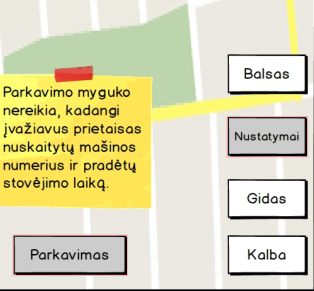
\includegraphics[scale=0.5]{img/def1}
	\caption{Navigacijos perpildymas \label{fig:def1}}
\end{figure}

\begin{figure}[H]
    \centering
    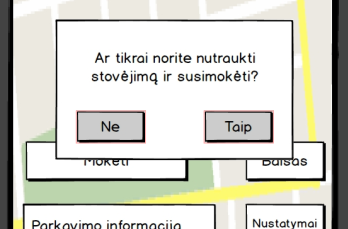
\includegraphics[scale=0.5]{img/def2}
	\caption{Persidengiantys langai \label{fig:def2}}
\end{figure}

\begin{figure}[H]
    \centering
    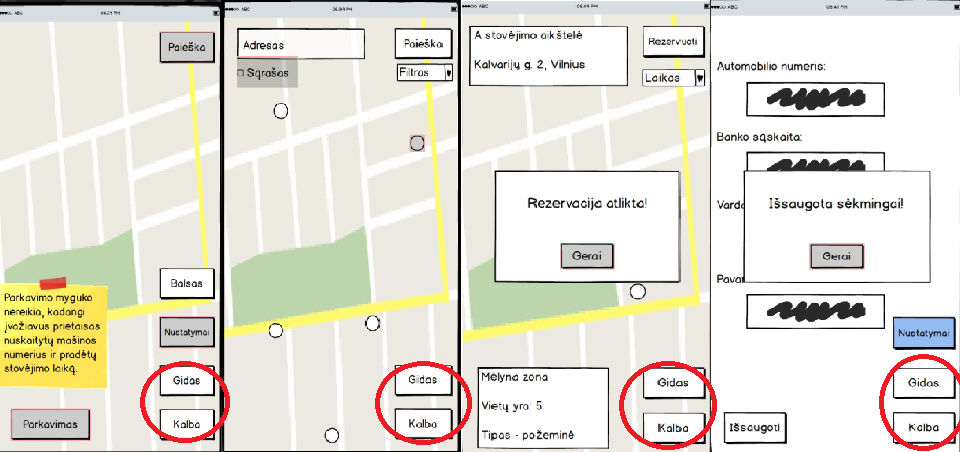
\includegraphics[scale=0.5]{img/def3}
	\caption{Nenaudingi mygtukai \label{fig:def3}}

\end{figure}

\begin{table}[H]\footnotesize
  \centering
  \caption{Tobulinimo galimybės}
  \begin{tabular}{|p{.05\textwidth}|p{.4\textwidth}|p{.1\textwidth}|p{.3\textwidth}|}
	\hline
	NR. & Trumpas aprašymas & Sunkumo įvertinimas & Rekomendacijos \\
	\hline
	1 & Per daug navigacijos pagrindiniame lange sukelia iššūkį vartotojams su mažais ekranais paspausti tinkamą mygtuką bei atrodo netvarkingai (\ref{fig:def1} pav.) & 5 & Išskaidyti į mažesnes dalis arba leisti vartotojui pašalinti, kai kurias dalis \\
	\hline
	2 & Persidengianti langai sukuria neaiškumų, kurie gali atbaidyti vartotojus nuo naudojimos programėle sukeliant baime paspausti ,,ne tą ką reikia'' (\ref{fig:def2} pav.)& 4 & Iškelti pagrindinius langus į viršų paslepiant žemesnius arb iš viso panaiktinti apatinius langus, kurie nėra esminiai \\
	\hline
	3 & Perteklinis mygtukų perpanaudojimas, atėma labai daug ekrano erdvės, tačiau nepriduoda funkcionalumo, šiuo atvėju tie mygtukai dar yra nėra dažnai spaudomi (\ref{fig:def3} pav.) & 3 & Retai naudojamo funkcionalumo mygtukus nedėti visuose languose, o tik tam tikruose pvz.(Nustatymai)\\
	\hline
	4 & Labai maži pagrindinio funkcionalumo mygtukai, sukelia nepatogumu ne tik spaudžiant, bet ir skaitant & 2 & Pagrindinius mygtukus padidinti, o sumažinti neaktualius \\
	\hline
	5 & Per daug patvirtinimo langų, sunkina darba vartotojui, taip pat įpratina kuo greičiau sutikti neskaitant ir taip gali pakenkti naudojimosi kokybe & 1 & Įdėti kai kurias žinutes į patį langą. \\
	\hline
  \end{tabular}
  \label{tab:defects}
\end{table}

\subsubsection{Pažintinė peržvalga}
\begin{itemize}
	\item Užduotis: susimokėti už parkavimą.

	\item Įprastas scenarijus:
		\begin{itemize}
			\item Turėti metalinių pinigų
			\item Išlipti iš mašinos
			\item Užrakinti mašiną
			\item Priejus prie parkomato spėti, kiek stovėsi laiko
			\item Susikaičiuoti, kiek reikia įdėti pinigų
			\item Įdėti pinigus 
			\item Paspausti žalią mygtuką
			\item Pasiimti čeki
			\item Grįžti prie mašinos
			\item Atrakinti mašiną
			\item Padėti čekį po langų
			\item Vėl užrakinti mašiną
		\end{itemize}
		
	\item Pateikiamas sprendimas:
	
		\begin{figure}[H]
			\centering
			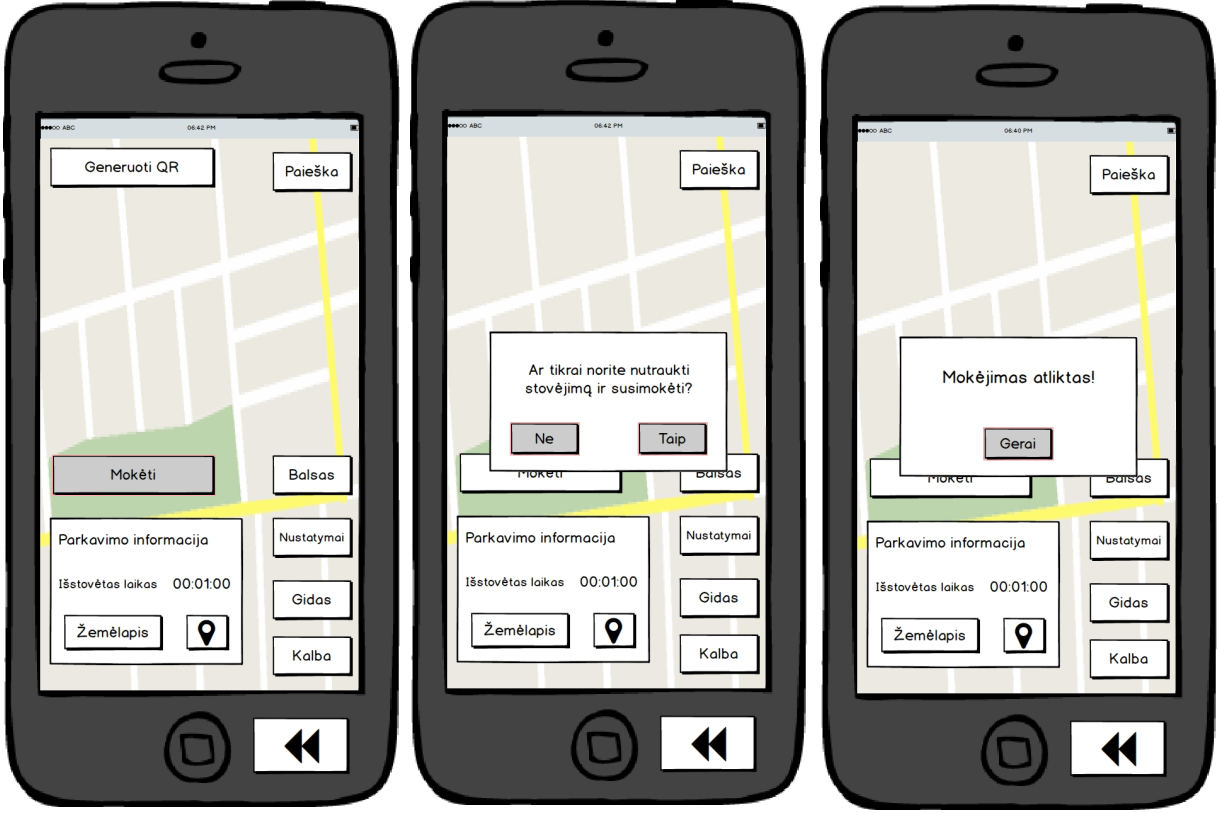
\includegraphics[scale=0.5]{img/pav4}
			\caption{Parkavimo apmokėjimas \label{fig:pav4}}
		\end{figure}
	
	\item Žingsniai:
		\begin{enumerate}
			\item Žingsnis. Išvažiuodami paspaudžiame mokėti
				\begin{itemize}
					\item Neįmanoma suklysti, nes tik vienas tinkamas mygtukas.
					\item Visą laiką matome, kiek prastovėjom ir kiek reikės sumokėti.
					\item Atsakas. Atsiras langas klausiantis patvirtinimo.
				\end{itemize}
			\item Žingsnis. Patvirtiname pasirinkimą
				\begin{itemize}
					\item Yra paaiškinamas kitas veiksmas ir paklausiama ar tinka.				
					\item Žinome ką paspaudžiame.				
					\item Atsakas. Iššoka sėkmingo apmokėjimo pranešimas. 
				\end{itemize}
		\end{enumerate}
\end{itemize}

\subsection{Vytauto Žilino maketo vertinimas}
,,ParQR'' komandos narys Vytautas Žilinas sukūrė inovatyvaus tipo sąsajos (interfeiso) maketą su pagrindiniais vartotojo siekiais bei daliniu funkcionalumu.

\subsubsection{Euristinis vertinimas}
Šiame skyriuje yra pateikta skyriaus ,,Metodas'' euristinio tikrinimo ataskaita.
Lentelėje 2 pateikta informacija apie tikrinimo aplinką.


\begin{table}[H]\footnotesize
  \centering
  \caption{Tikrinimo aplinka}
  {\begin{tabular}{|p{.2\textwidth}|p{.5\textwidth}|}
	\hline
	Vertintojas & Miglė Vaitulevičiūtė\\
	\hline
	Amžius & 20 \\
	\hline
	Lytis & Moteris \\
	\hline
	Naršyklė & Chrome \\
	\hline
	OS & Windows 10 \\
	\hline
	Vaizduoklio spalvos & 32 bitai \\
	\hline
	Skiriamoji geba & 1366x768 \\
	\hline
	Vaizduoklio dydis & 15.6 inches \\
	\hline
	Vertinimo data & 2017 10 26 \\
	\hline
	Vertinimo laikas & 15:00-16:00 \\
    \hline
  \end{tabular}}
  \label{tab:table example}
\end{table}

\subsubsubsection{Stiprybės}
Šiame skyriuje yra pateikta visi Vytauto Žilino sukurto maketo teigiami aspektai (1-3 pav.).
\vspace{5mm}

\begin{itemize}
\item Inovatyvi ir minimalistinė sąsaja (interfeisas)\par
\begin{minipage}{\linewidth}
\captionof{figure}[h]{Pradinis ekrano vaizdas}
\centering
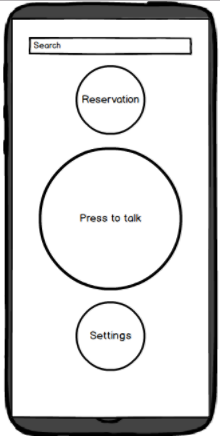
\includegraphics[width=5cm]{img/Good1}
\end{minipage}
\item Tinkamas kiekis informacijos nusakančios parkavimo rodiklius (kaina ir laikas)\par
\begin{minipage}{\linewidth}
\captionof{figure}[h]{Parkavimo rodikliai}
\centering
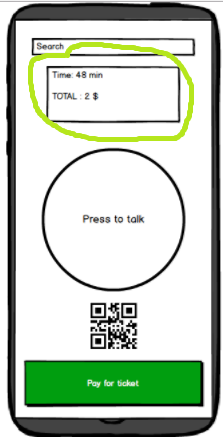
\includegraphics[width=5cm]{img/Good2}
\end{minipage}
\item Egzistuoja papildomas kelias - atšaukti ,,autoPay'' naudojimą\par
\begin{minipage}{\linewidth}
\captionof{figure}[h]{Pranešimas}
\centering
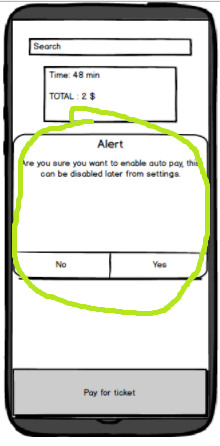
\includegraphics[width=5cm]{img/Good3}
\end{minipage}
\end{itemize}

\subsubsubsection{Tobulinimo galimybės}
Šiame skyriuje pateiktos Vytauto Žilino sukurto maketo esminės problemos (4-6 pav.).

\vspace{5mm}
\begin{itemize}
\item Neaiški QR kodo metafora, jog šis QR kodas yra mygtukas ir ant jo galima paspausti, kad toliau būtų galima vykdyti apmokėjimą.\par
\begin{minipage}{\linewidth}
\captionof{figure}[h]{QR kodo metafora}
\centering
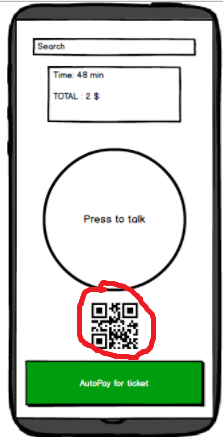
\includegraphics[width=5cm]{img/Bad1}
\end{minipage}
\item Neaiški rodyklės metafora, jog ji yra skirta apmokėti už stovėjimo laiką.\par
\begin{minipage}{\linewidth}
\captionof{figure}[h]{Rodyklės metafora}
\centering
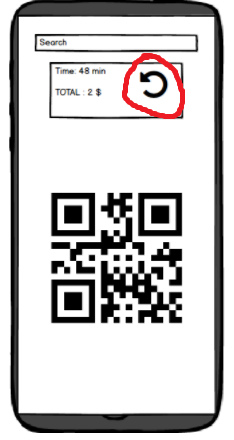
\includegraphics[width=5cm]{img/Bad2}
\end{minipage}
\item Mokant už parkavimo laiką yra per daug validacinių langų, jie erzina vartotoją.\par
\begin{minipage}{\linewidth}
\captionof{figure}[h]{Validacijos pranešimai}
\centering
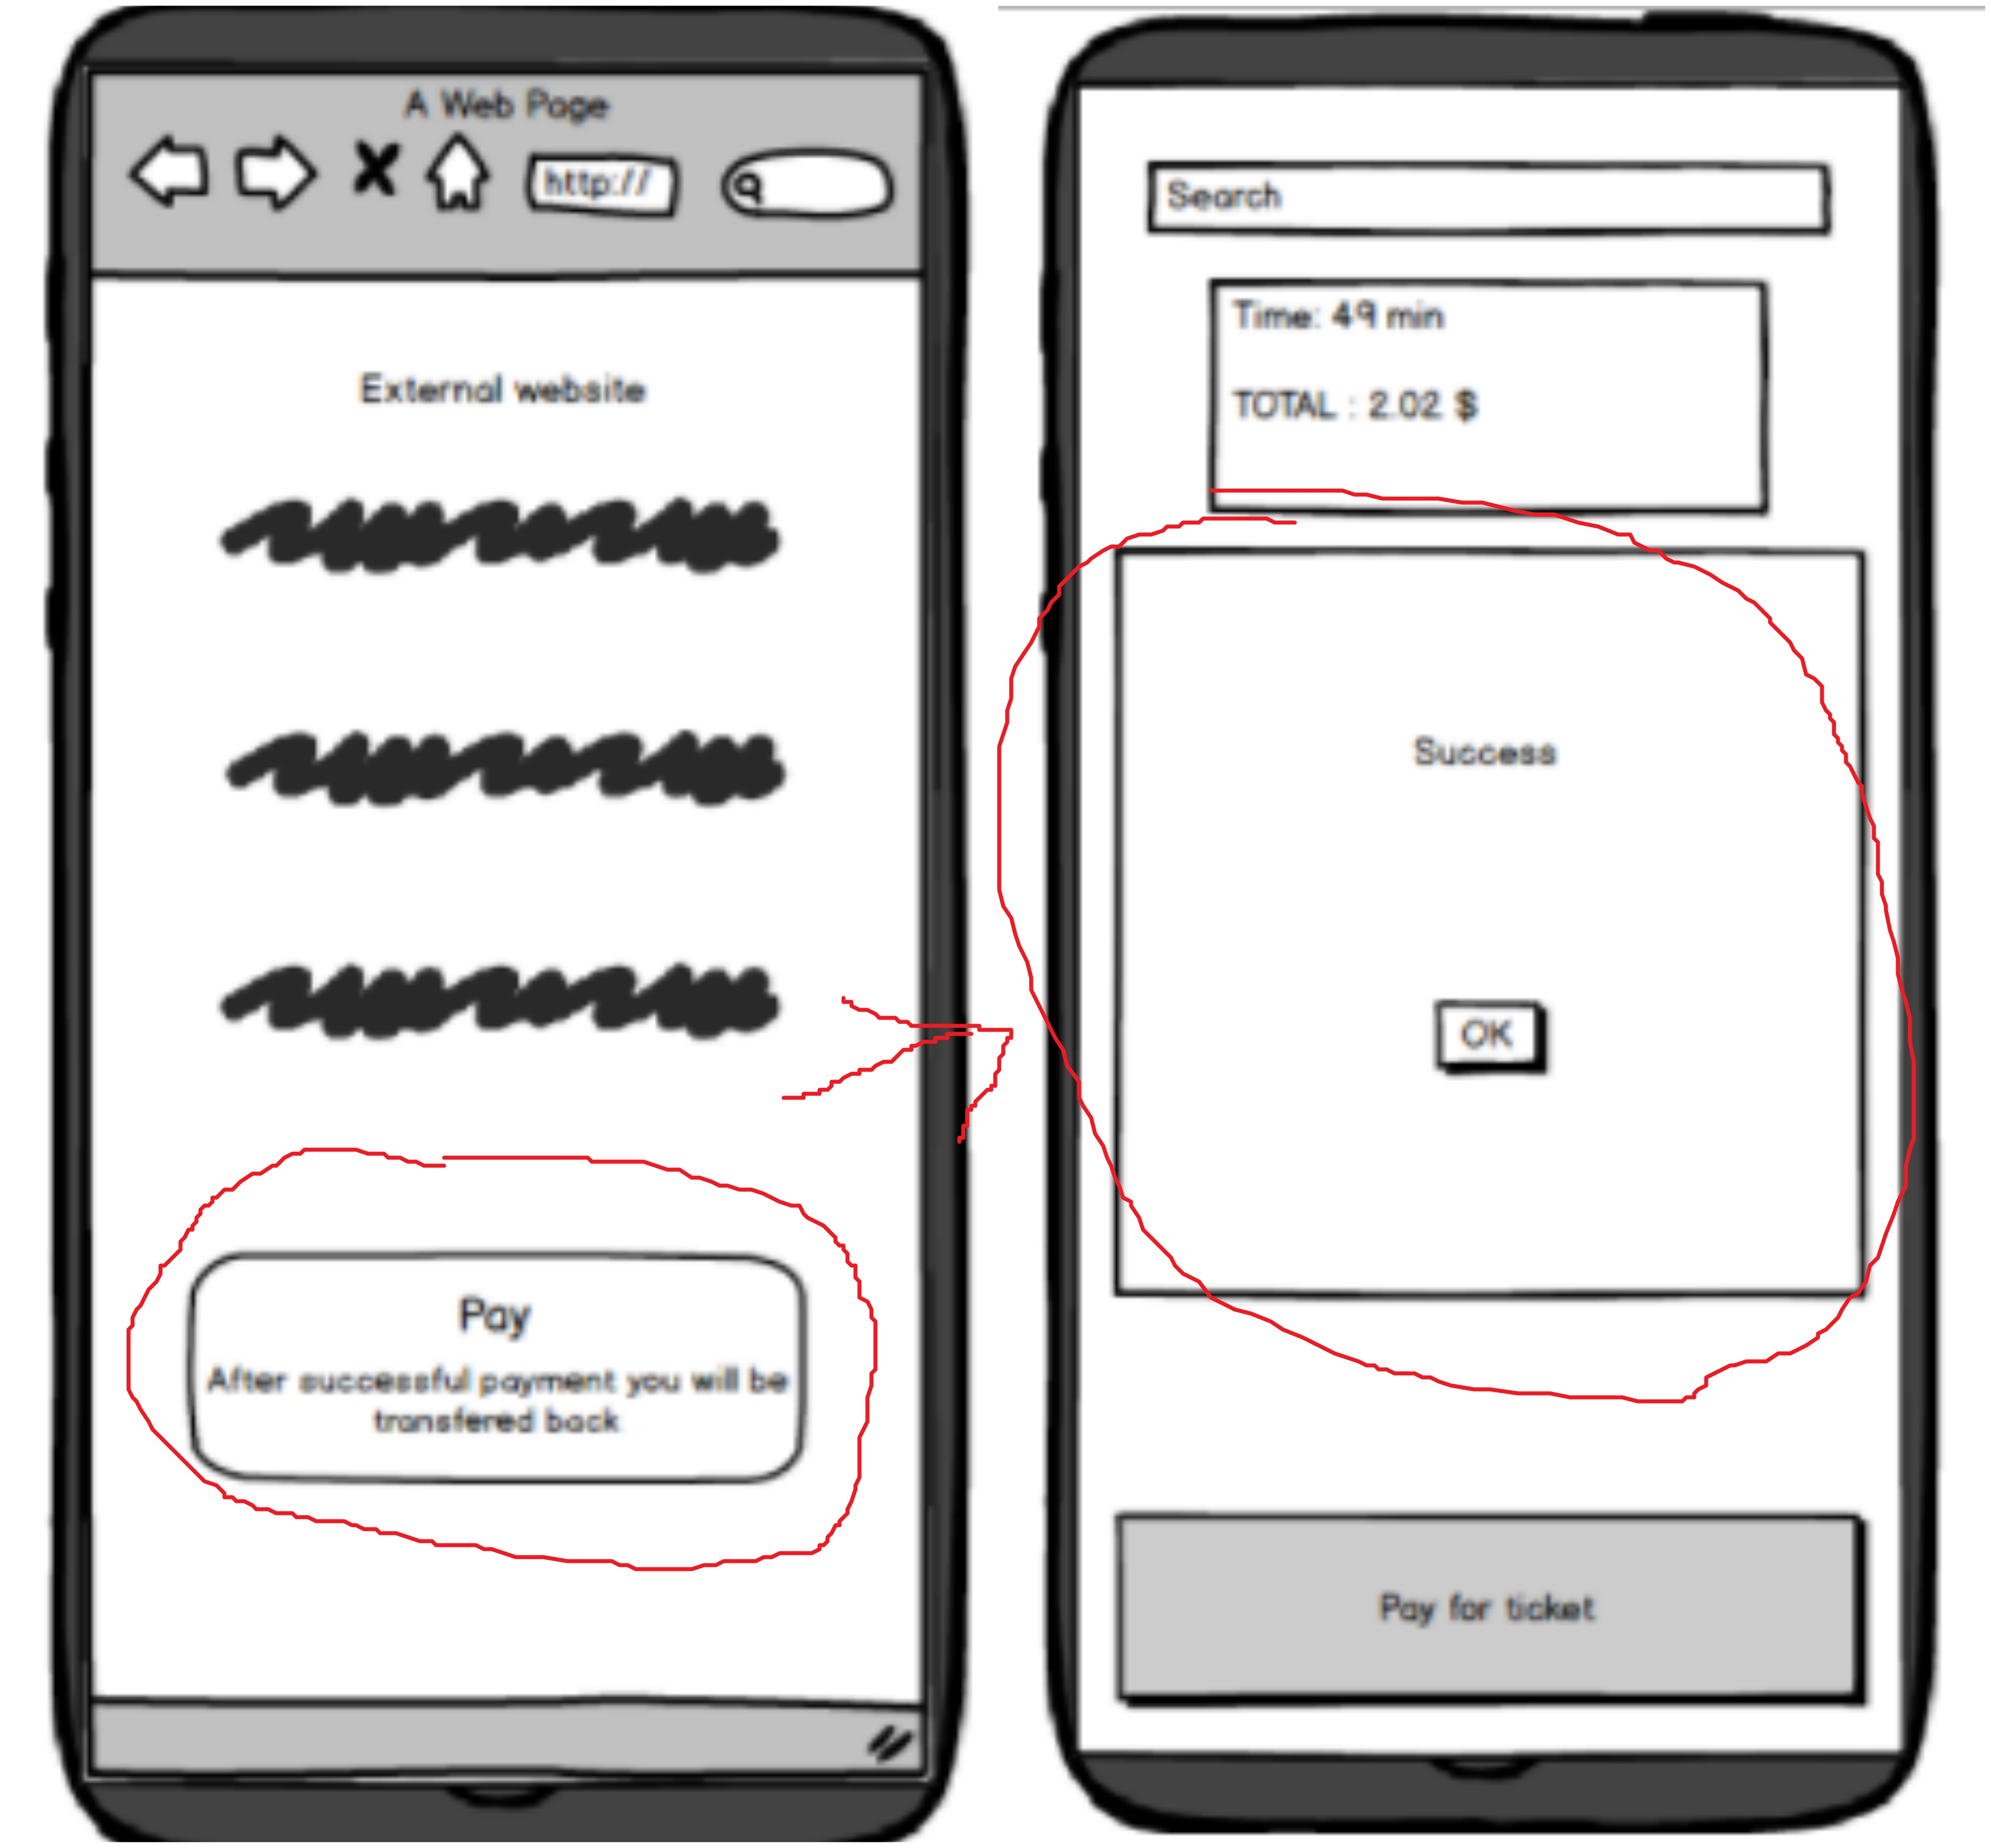
\includegraphics[width=5cm]{img/Bad3}
\end{minipage}
\end{itemize}

\subsubsection{Pažintinė peržvalga}
Šiame skyriuje yra pateikta pagrindinės užduotys, kurios yra atvaizduotos Vytauto Žilino makete.


\begin{enumerate}
\item Užduotis - Sumokėti už išstovėtą laiką naudojantis ParQR programėle
\item Naudotojui įprastų veiksmų scenarijus
\begin{enumerate}
\item Paspaudžia ant mokėjimo mygtuko
\item Pasirenkama per kokį banką mokama
\item Gauna mokėjimo patvirtinimą
\end{enumerate} 
\item Paspaudžia ant mokėjimo mygtuko
\begin{itemize}
\item Vartotojas žino, ką ir kaip jam veikti, nes programėlės apačioje pateiktas mygtukas ,,Pay for ticket''.
\item Vartotojas atlikęs teisingą veiksmą sužino, kad priartėjo prie tikslo, kadangi programėlės ekranas pasikeičia į kitą užduoties vykdymo žingsnį.
\end{itemize}
\item Pasirenkama per kokį banką mokama
\begin{itemize}
\item Vartotojas žino, ką ir kaip jam veikti, nes programėlės viduryje pateiktas sąrašas bankų pavadinimų, kuriuos galima paspausti.
\item Vartotojas atlikęs teisingą veiksmą sužino, kad priartėjo prie tikslo, kadangi programėlės ekranas pasikeičia į mokėjimo patvirtinimą.
\end{itemize}
\item Gauna mokėjimo patvirtinimą
\begin{itemize}
\item Vartotojas žino, ką ir kaip jam veikti, nes programėlės apačioje yra pateiktas pranešimas su užduoties atlikimo teigniu.
\item Vartotojas atlikęs teisingą veiksmą sužino, kad priartėjo prie tikslo, kadangi programėlės ekrane atsiranda pranešimas su informacija.
\end{itemize}
\end{enumerate}

\section{Išvados}

Iš Miglės Vaitulevičiūtės maketo mes pernaudosim nustatymų menių, kadangi tai labai veiksmingas vartotojo atminties apkrovos minimizavimas. Taip pat bus funkcionalus mygutkas atgal, kadangi jis labai stipriai pagerina valdomumą. Bei pus panaudota artimiausiu parkavimų aikštelių paieška, kadangi ji relalizuoja tinkamumą užduočiai.

\begin{figure}[H]
    \centering
    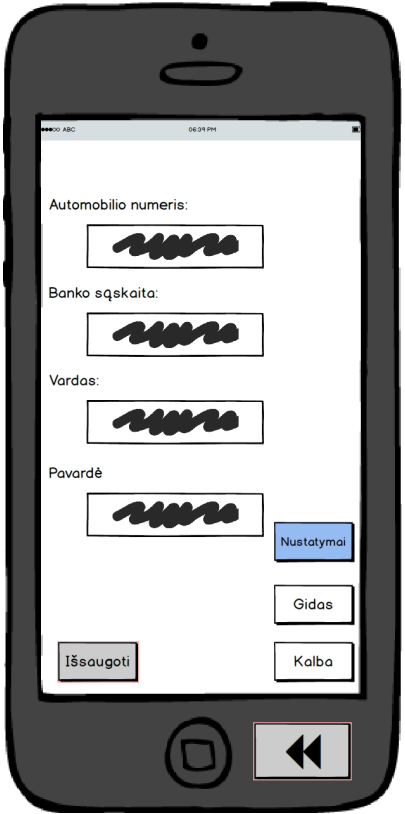
\includegraphics[scale=0.5]{img/mig1}
	\caption{Nustatymų menių \label{fig:mig1}}
\end{figure}

\begin{figure}[H]
    \centering
    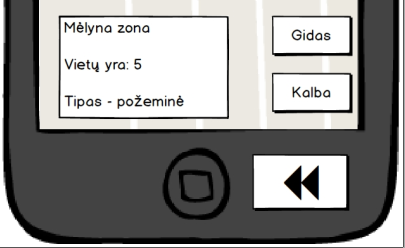
\includegraphics[scale=0.5]{img/mig2}
	\caption{Funkcionalus mygtuka \label{fig:mig2}}
\end{figure}

\begin{figure}[H]
    \centering
    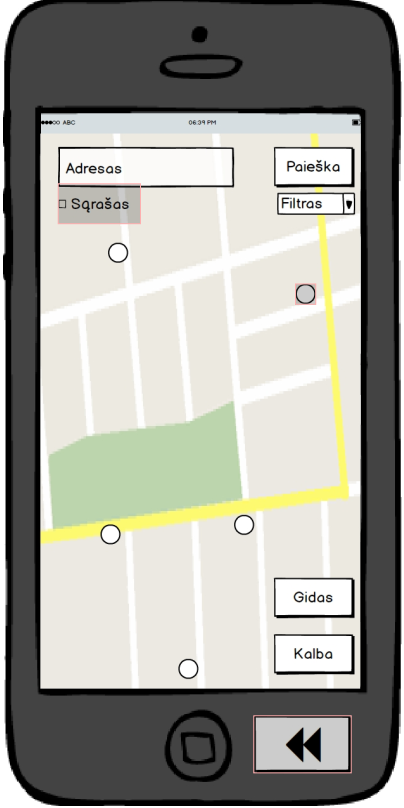
\includegraphics[scale=0.5]{img/mig3}
	\caption{Artimiausios aikštelės \label{fig:mig3}}
\end{figure}

Iš Vytauto Žilino maketo bus pernaudotas minimalistinis meniu, nes, mūsų nuomone, jis yra pakankamai funkcionalus, ir estetiškai malonus. Taip pat bus perimta galimybė įjungti greitus apmokėjimus, nes tai stiprai pagerina naudojimosi lankstumą. Bei bus paimta ir patobulinta QR kodo implementacija.


\begin{figure}[H]
    \centering
    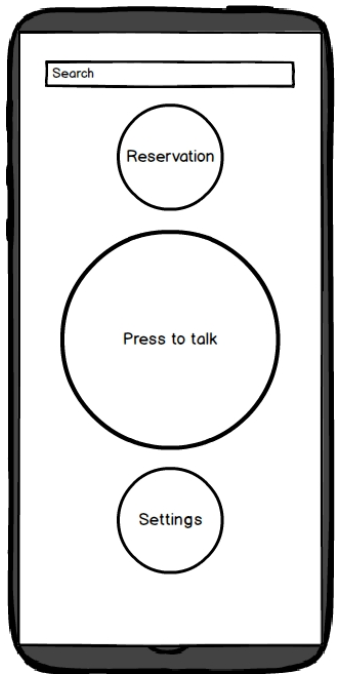
\includegraphics[scale=0.5]{img/vyt1}
	\caption{Nustatymų menių \label{fig:vyt1}}
\end{figure}

\begin{figure}[H]
    \centering
    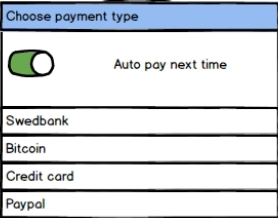
\includegraphics[scale=0.5]{img/vyt2}
	\caption{Funkcionalus mygtuka \label{fig:vyt2}}
\end{figure}

\begin{figure}[H]
    \centering
    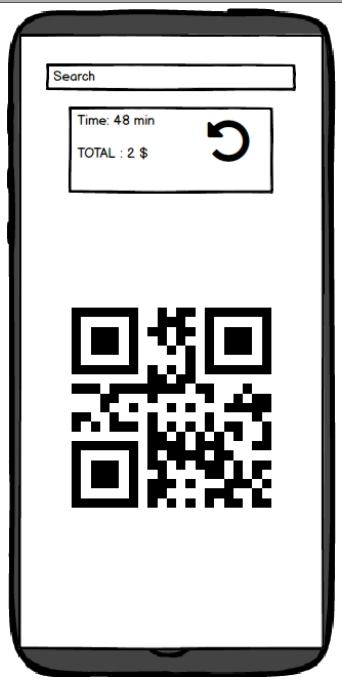
\includegraphics[scale=0.5]{img/vyt3}
	\caption{Artimiausios aikštelės \label{fig:vyt3}}
\end{figure}

\end{document}
